
%(BEGIN_QUESTION)

\large \textbf{Praktisk øving på brødbrett - Enkel motstand}
\normalsize 
\vskip 10pt 
I denne øvingen skal du bruke et koblingsbrett for å koble en motstand til en 24V industristrømforsyning.

\vskip 10pt 
Koblingsbrettet brukes for å koble sammen komponentene.
$$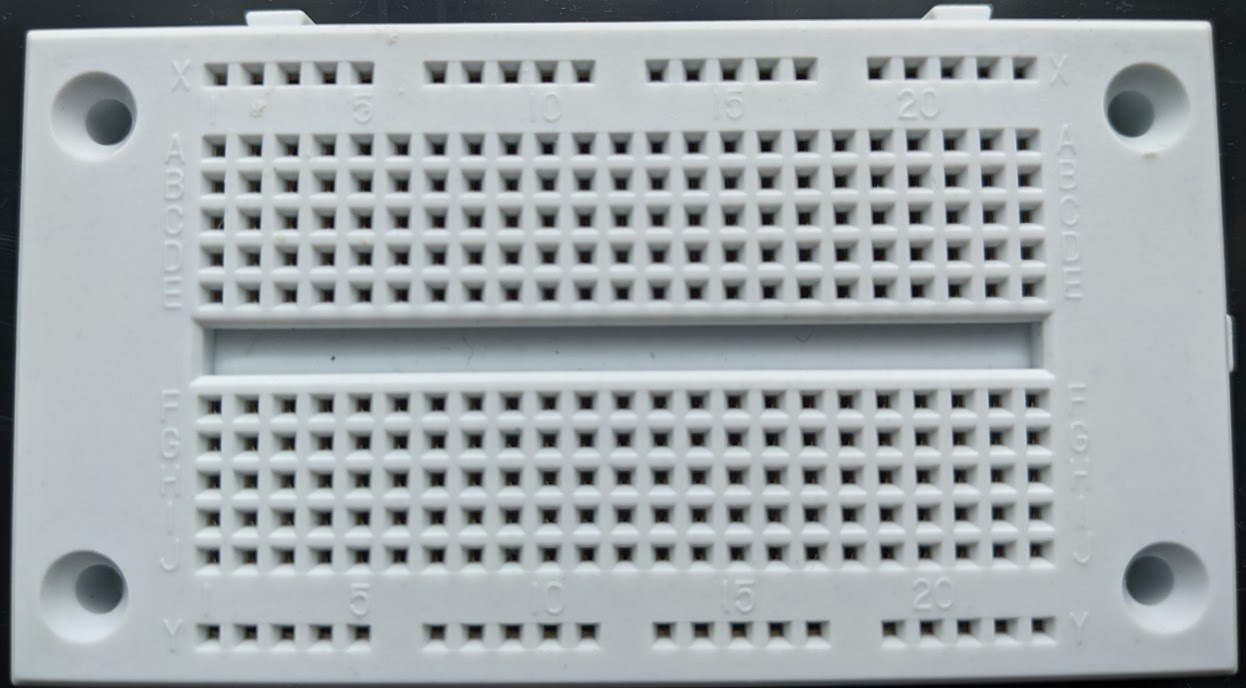
\includegraphics[width=10cm]{breadboard.jpg}$$


\vskip 10pt 
\large \textbf{Utstyr du trenger}

\vskip 10pt 
\begin{itemize}[noitemsep]

\item 9V batteri
\item Koblingsbrett
\item Isolert ledning
\item Resistans på $3.3k\Omega$
\item Amperemeter
\item Voltmeter
\item Ohmmeter
\end{itemize}


\large \textbf{Kretsen}
\normalsize
\vskip 10pt 
En motstand på $R_{1}=1.2k\Omega$ til strømforsyningen. 

\vskip 10pt 
Teorioppgaver:
\begin{itemize}[noitemsep]
\item 
Tegn kretsen
Regn ut strømmen $I$ i kretsen
Forklar hvordan et voltmeter virker
Forklar hvordan et amperemeter virker
Forklar hvordan et ohmmeter virker.
\end{itemize}

Praktiske oppgave:
\begin{itemize}[noitemsep]
\item koble opp kretsen
\item Mål resistansen $R_{1}$
\item Mål spenningen over resistansen $R_{1}$
\item Koble inn et amperemeter og mål strømmen igjennom $R_{1}$
\end{itemize}



 


\underbar{file i04876}
%(END_QUESTION)





%(BEGIN_ANSWER)


%(END_ANSWER)





%(BEGIN_NOTES)



%INDEX% Electronics review: series-parallel circuits

%(END_NOTES)


